\documentclass[12pt,a4paper]{report}
\usepackage{fontspec}

%\setmainfont{???}
\usepackage{amsmath}
\usepackage{amsfonts}
\usepackage{amssymb}
\usepackage{graphicx}
\usepackage[margin=1in]{geometry}
\usepackage{tcolorbox}
\usepackage{tikz}
\usepackage{minted}
\usepackage{svg}
\usetikzlibrary{calc}

\title{DCE assignment - 2}

\begin{document}
\begin{titlepage}
    \centering
    \begin{tikzpicture}[remember picture, overlay]
        \draw[line width = 2pt] ($(current page.north west) + (1in,-1in)$) rectangle ($(current page.south east) + (-1in,1in)$);
    \end{tikzpicture}
\vspace*{2in}

{\Large \textsc {Digital Communication Engineering} \\ [2em]
\Large \textsc {Assignment 2}
}
\vfill
\begin{flushright}

    \begin{tcolorbox}[colback=white, colframe=black,width=6.5cm,before skip=0pt,right skip=.5cm,bottom=0cm,top=.5cm,left=20pt]
\textit{\underline{Submitted by}:} \\[7pt]
       \hspace*{20pt} Roopesh O R \\
       \hspace*{20pt} Roll. no: 31 \\
       \hspace*{20pt} Reg. no: 20323085 \\
    \end{tcolorbox}

\end{flushright}
\end{titlepage}
\raggedbottom
\section*{Question 1}
 Implement a TDM system using MATLAB code / SIMULINK model.
 \subsection*{Code}
\begin{minted}{matlab}
clearvars; close all;
t = linspace(0, 2, 1000);
signals = {
    sin(2*pi * t);
    2*cos(t * 2*pi) + sin(t * 2*pi);
    2*cos(t * pi);
};
signalNames = {"m1", "m2", "m3"};
signalCols = {"blue", "red", "#058217"};
N = length(signals); % no of signals to mux
% contains all PAM modulated signals
pamMods = zeros(N, length(signals{1}));
% no of data points each each signal can tx at a time (pulse width)
Tsignal = 15;
Tspacing = 3; % spacing between each signal
% create N shifted pulse trains each with pulse width Tsignal
MuxPulses = kron(eye(N), [ones(1, Tsignal), zeros(1, Tspacing)]);
for i=1:N
    pamMods(i, :) = pamMod_Demod(signals{i}, MuxPulses(i, :));
end
tdm = sum(pamMods); % sum all PAMs along column axis

demuxed = zeros(N, length(tdm));
for i=1:N
    demuxed(i, :) = pamMod_Demod(tdm, MuxPulses(i, :));
end

subplot(3, 2, 1); hold on
for i = 1:N
    plot(t, signals{i}, "Color", signalCols{i});
end
legend(signalNames);
title("Signals to mux");
xlabel("t"); ylabel("Amplitude");

subplot(3, 2, 3); hold on
for i=1:N
    stairs(t, pamMods(i, :), "Color", signalCols{i});
end
title("individual PAM");
xlabel("t"); ylabel("Amplitude");
legend(signalNames);

subplot(3, 2, 5); stairs(t, tdm);
title("TDM signal");
xlabel("t"); ylabel("Amplitude");
for i=1:N
    subplot(3, 2, 2*i);
    stairs(t, demuxed(i, :), "Color", signalCols{i});
    title("Demuxed signal: " + signalNames{i});
end
ylim(findobj(gcf, 'Type', 'Axes'), [-3 3]);

function y = pamMod_Demod(x, seq)
    L = ceil(length(x) / length(seq));
    sq = kron(ones(1, L), seq);
    sq = sq(1:length(x)); % make length same
    y = x .* sq;
end
\end{minted}

\subsection*{Output waveforms}
\begin{figure*}[!h]
    \includesvg[inkscapearea=drawing, width=\textwidth]{tdm}
\end{figure*}

\section*{Question 2}
Create a MATLAB code to simulate Delta modulation and demodulation system.

\subsection*{Code}

\begin{minted}{matlab}
clearvars; close all;

fm = 1; % highest msg freq
fs = 50; % sampling freq
t = 0:1/fs:1;

msg = 3 * sin(2*pi*t*fm);
dy = .4; % delta size

%%%% Modulation
accumulator = 0;
len = length(t);
deltaMod = repelem(-1, len);
accumulated = zeros(1, len);
for i = 1:len
    if (msg(i) > accumulator)
        deltaMod(i) = 1;
        accumulator = accumulator + dy;
    else
        accumulator = accumulator - dy;
    end
    accumulated(i) = accumulator;
end

subplot(3, 1, 1);
hold on
plot(msg);
stairs([accumulated, 0]);
xlim([1, len]);
xlabel("sample");
ylabel("Amplitude");
legend(["Input signal", "Accumulator"]);
title("Input signal & accumulator");

subplot(3, 1, 2);
stairs([deltaMod, 0]);
title("Delta modulation & corresponding bitstream");
xlabel("samples");
for i = 1:len
   text(i + 0.2, 0, string((deltaMod(i) + 1)/2));
end
xlim([1, len+1]);
ylim([-1.2, 1.2]); yticks([-1, 1])

%%%% Demodulation
N = length(deltaMod);
accum = zeros(1, N);
for i = 2:N
    accum(i) = accum(i-1) + dy * deltaMod(i-1);
end

% apply low pass
[b, a] = butter(3, fm / fs * 10);
y = filter(b, a, accum);

subplot(3, 1, 3);
hold on;
stairs(accum);
plot(y);
xlim([1, N]);
title("Demodulated output");
legend(["Accumulator", "Filter output"])
xlabel("samples");
ylabel("Amplitude");
\end{minted}

\subsection*{Output waveforms}
\begin{figure*}[!h]
    \includesvg[inkscapearea=drawing, width=\textwidth]{dm}
\end{figure*}

\section*{Question 3}
Implement BPSK, BASK and BFSK modulation using MATLAB code/ SIMULINK model.

\subsection*{Code}
\begin{minted}{matlab}
clearvars; close all;

Tb = 1;   % symbol period
fs = 500; % freq at which basis fxs are sampled
t = linspace(0, Tb, fs);

msgbits = [1 0 1 1 0 1 0];
N = length(msgbits);

% basis functions
fc1 = 5;
fc2 = 8;
s1 = sqrt(Tb/2) * cos(2*pi*fc1.*t);
s2 = sqrt(Tb/2) * cos(2*pi*fc1.*t+pi);
s3 = sqrt(Tb/2) * cos(2*pi*fc2.*t);

msgsampled = kron(msgbits, ones(1, fs));
bask = kron(msgbits, s1);
bpsk = kron(msgbits, s1) + kron(~msgbits, s2);
bfsk = kron(msgbits, s1) + kron(~msgbits, s3);

tiledlayout(4, 1);
t = linspace(0, Tb*N, fs*N);
plot_(t, msgsampled, "Message");
for i=1:N
    text(i-0.5, 0.5, string(msgbits(i)));
end
plot_(t, bask, "BASK");
plot_(t, bpsk, "BPSK");
plot_(t, bfsk, "BFSK");

function plot_(t, fx, title_)
    nexttile;
    plot(t, fx);
    k = (max(fx) - min(fx)) * 0.2;
    ylim([min(fx) - k, max(fx) + k]);
    title(title_);
    xlabel("t");
    ylabel("Amplitude");
end

\end{minted}

\subsection*{Output waveforms}
\begin{figure*}[!h]
    \includesvg[inkscapearea=drawing, width=\textwidth]{bsk}
\end{figure*}
\end{document}